% Section content template for individual Educative lessons
% This file contains the actual content for a specific section
% Generated from Educative API section content

% Section: Use Case Diagram for the Restaurant Management System
% Section ID: 6482479776268288
% Section Slug: use-case-diagram-for-the-restaurant-management-system
% Generated: 2025-12-14T12:23:00.239089

Let's build the use case diagram for the restaurant management system and understand the relationship between its different components. First , we'll define the different elements of our restaurant, followed by the complete use case diagram of the system.

\subsection{System}\label{xaJUmYRjdS5aQ6FH2EsMB}
\\
Our system is a restaurant management system.

\subsection{Actors}\label{WJjT6kjYegHoXrd54bxdE}
\\
Let's define the main actors of our restaurant management system.

\subsubsection{Primary actors}\label{wBsFP5uLmDkqwS1l_Z28n}

\begin{itemize}
\item
\protect\phantomsection\label{WouBZyJ5T5felzIs_c0ZC}
\textbf{Customer:} This is the restaurant's primary actor who can view the menu, place orders, make a reservation, and make payments.
\item
\protect\phantomsection\label{lrgy0egSv6DGdij3WJZum}
\textbf{Receptionist:} This actor is responsible for reserving tables and updating the table reservation status.
\item
\protect\phantomsection\label{0jO2tLUERdbT8kGwjHSlU}
\textbf{Server:} This actor takes the order from the customer and processes the payment.
\item
\protect\phantomsection\label{875SBRNrh1Jy9iGLvU7YS}
\textbf{Manager:} This actor manages each branch's menu and table configuration.
\end{itemize}

\subsubsection{Secondary actor}\label{8gO7hU5GmukeTxCBm8M19}

\begin{itemize}
\item
\protect\phantomsection\label{Ojbcy61MkxOVo7QBKX8NJ}
\textbf{System:} This can automatically notify customers when their reservation time approaches and update table statuses whenever a bill is paid or a reservation is made.
\end{itemize}

\subsection{Use cases}\label{XzyFtETow34hBYc5yBNZO}
\\
This section will define the restaurant management system's use cases. We 've listed them according to their respective interactions with a particular actor.

\subsubsection{Customer}\label{GPh57H1QxJPPBSjxUI1AT}

\begin{itemize}
\item
\protect\phantomsection\label{ThcyiGUcsf9vfdWo9uKl_}
\textbf{View menu:} To browse food items and prices.
\item
\protect\phantomsection\label{3SKDMftGkvyxhoqtjqN3U}
\textbf{Make reservation:} To book a table.
\item
\protect\phantomsection\label{oElh6x6x6PEeUYpzlj1ww}
\textbf{Cancel reservation:} To cancel an existing reservation.
\item
\protect\phantomsection\label{A3PSwFQrcWvSXKqvdLEqS}
\textbf{Place order:} To order food.
\item
\protect\phantomsection\label{A1KKAmy3bmNeynLdCoqlY}
\textbf{View order:} To check order status or details.
\item
\protect\phantomsection\label{G0u2zEXIVkGiL2rS2wAlz}
\textbf{Receive notification:} To receive a notification when the reservation time approaches.
\item
\protect\phantomsection\label{2cqLaRQ2rXTWLTkXX_4F2}
\textbf{Pay bill:} To complete payment using cash or a card.
\item
\protect\phantomsection\label{Qt6iuvdptA9ENNh14ioHK}
\textbf{Search available tables:} To check table availability in real time.
\item
\protect\phantomsection\label{n4YX-xQZ3A7Oix3e341rw}
\textbf{Request Bill Details:} To get the details to pay the bill.
\end{itemize}

\subsubsection{Manager}\label{jgQsx495o6YJeOs4ce3vR}

\begin{itemize}
\item
\protect\phantomsection\label{5SGHT-CP0vpDz7Rw-SgeX}
\textbf{Add/modify menu section:} To manage food categories.
\item
\protect\phantomsection\label{_JZ66uNrzo9X8_sIN7jDQ}
\textbf{Add/modify menu item:} To manage individual food items.
\item
\protect\phantomsection\label{HjCiYsiJg2OsqkMC9UfKi}
\textbf{Add/update table configuration:} To define branch-specific table layouts.
\item
\protect\phantomsection\label{zDsKv5REEl-dg4h41iT51}
\textbf{View menu:} To access the menu for decision-making or management.
\end{itemize}

\subsubsection{Receptionist}\label{fA9KqAqMr9W1m9H0SJjck}

\begin{itemize}
\item
\protect\phantomsection\label{Qt6iuvdptA9ENNh14ioHK}
\textbf{Search available tables:} To check table availability in real time.
\item
\protect\phantomsection\label{-F8HXIsH_SrwmAZCqnrOQ}
\textbf{Make reservation:} To book a table for a customer.
\item
\protect\phantomsection\label{MzsGDsfxMHckXuqGziL59}
\textbf{Cancel reservation:} To cancel an existing reservation.
\item
\protect\phantomsection\label{Vqa1_6BgGIILAR9Z5QIti}
\textbf{Receive notification:} To receive notification when a reservation time approaches.
\item
\protect\phantomsection\label{r2iqcjXCyAVe9sg1rVk33}
\textbf{Modify reservation:} To modify an existing reservation.
\end{itemize}

\subsubsection{Server}\label{VhWc7GqKkysxdubbw58pa}

\begin{itemize}
\item
\protect\phantomsection\label{nXS_EVZr91rywjwmn7lke}
\textbf{View menu:} To assist with customer ordering.
\item
\protect\phantomsection\label{GMG2ePiZcHhnKg394b7og}
\textbf{Take order:} To take and enter customer orders.
\item
\protect\phantomsection\label{eagqK_ewax4kiut9GRnMC}
\textbf{Fetch order list:} To view assigned or active orders.
\item
\protect\phantomsection\label{XbJEmrfWki289-B-wthUI}
\textbf{Replace meal item:} To substitute an item in an existing order.
\item
\protect\phantomsection\label{PnmKkc_gy4eoIMOVQpiIA}
\textbf{Generate bill:} To calculate the total bill against the food order.
\end{itemize}

\subsubsection{System}\label{z9PPBMZ9Xu_c2IWq7IroM}

\begin{itemize}
\item
\protect\phantomsection\label{SvP90YNp4nilJTnz-knW8}
\textbf{Send notifications:} To automatically notify customers when their reservation time approaches.
\item
\protect\phantomsection\label{2Q65wCmiRkEeACW7yZ2iu}
\textbf{Update table statuses:} To handle automatic updates of table availability.
\end{itemize}

\subsection{Relationships}\label{bCvJbxBPuP8uzbDVF99ff}
\\
This section describes the relationships between and among actors and their use cases.

\subsubsection{Associations}\label{mJxo-lPAEt-ItZWTmZR1m}
\\
The table below shows the association relationship between actors and their use cases.

\begin{table}[htbp]
\centering
\small
\adjustbox{max width=\textwidth}{
\begin{tabular}{|p{0.238\textwidth}|p{0.254\textwidth}|p{0.207\textwidth}|p{0.250\textwidth}|}
\hline
\textbf{Customer} & \textbf{Receptionist} & \textbf{Server} & \textbf{Manager} \\
\hline
\hline
View menu & Search available tables & View menu & Add/modify menu section \\
\hline
Make reservation & Make reservation & Take order & Add/modify menu item \\
\hline
Pay bill via cash/card & Update/cancel reservation & Fetch order list & Add/update table configuration \\
\hline
Cancel reservation & Receive notification & Replace meal item & \hfill\break \\
\hline
Place order & \hfill\break & Generate bill & \hfill\break \\
\hline
View order & \hfill\break & \hfill\break & \hfill\break \\
\hline
Receive notification & \hfill\break & \hfill\break & \hfill\break \\
\hline
Search available tables & \hfill\break & \hfill\break & \hfill\break \\
\hline
Request Bill Details & \hfill\break & \hfill\break & \hfill\break \\
\hline
\end{tabular}
}
\end{table}

\subsubsection{Include}\label{fjUBo1nxSowcXu6OAt5BE}
\\
When a customer wants to make a reservation, the system checks for available tables before confirming the booking. Additionally , the system updates the table status once the reservation is made.

\begin{itemize}
\item
\protect\phantomsection\label{3qbeO6i1qsEtptdSDVrbh}
The \textbf{Make reservation} use case includes \textbf{search available tables} and \textbf{update table status} use cases\textbf{.}
\end{itemize}
\\
When a customer cancels their reservation, the system updates the table status to reflect the availability.

\begin{itemize}
\item
\protect\phantomsection\label{MWGchWngE_9qYhR_7bRmf}
The \textbf{Cancel reservation} use case includes \textbf{Update table status} use case.
\end{itemize}
\\
When staff take a customer's order, they must first view the current menu to select items.

\begin{itemize}
\item
\protect\phantomsection\label{VmWE2yzdVJzcpgHOnFL-h}
The \textbf{Take order} use case includes \textbf{View menu} use case.
\end{itemize}
\\
When a customer pays the bill, the system marks the table as paid and updates its status accordingly.

\begin{itemize}
\item
\protect\phantomsection\label{6W0f0ANf7uRwetkNDyzoU}
The \textbf{Pay bill} use case includes \textbf{Update table status} use case.
\end{itemize}

\subsubsection{Extend}\label{NuiTDTp5eFMeuj4A-WBkA}
\\
Users can pay using cash or a card when they choose to process a payment.

\begin{itemize}
\item
\protect\phantomsection\label{WEM1oz3bBUWMAZk-ze-gV}
The \textbf{Process payment} use case extends to \textbf{Pay bill via cash} and \textbf{Pay bill via card} use case.
\end{itemize}
\\
When a user wants to change the details of an existing reservation, they modify the original booking.

\begin{itemize}
\item
\protect\phantomsection\label{Py-qdHtrK-PmwyZAKyJ-e}
The \textbf{Modify reservation} use case extends the \textbf{Make reservation} use case.
\end{itemize}

\subsection{Use case diagram}\label{WnC1r8IvpTO4EQa1omYy4}
\\
Here's the use case diagram of the restaurant management system:

\begin{figure}[htbp]
 \centering
 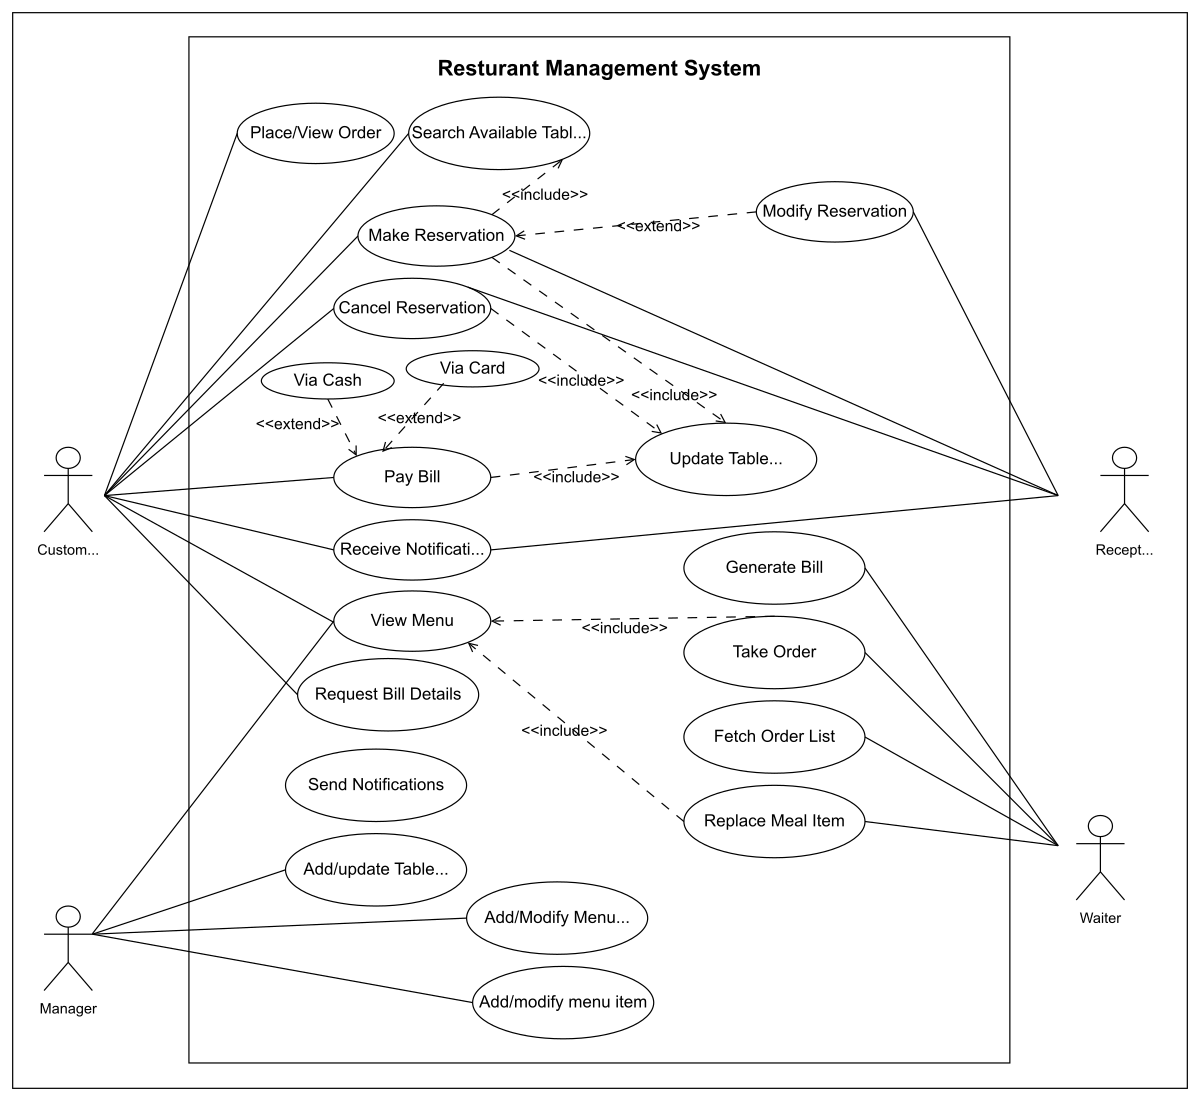
\includegraphics[width=0.5\textwidth]{Images/chapter_21/section_6482479776268288/6473777016602624.png}
 \caption{The use case diagram of the restaurant management system}
\end{figure}

In the next lesson, we'll discuss the class diagram with a detailed explanation of all classes and their relationship with each other.

% End of section content